% \documentclass{standalone}
% \input{../tikz_header}


% %\usetikzlibrary{hobby}


% \begin{document}



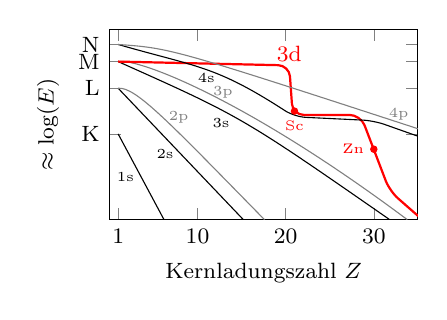
\begin{tikzpicture} 


  \begin{axis}
    [font=\footnotesize,
      ymin = 0, ymax = 1, xmin=0,  xmax=35,
      %ticks=none,
      width=55mm, height=40mm,
      xtick = {1, 10, 20, 30},
      xlabel = {Kernladungszahl $Z$},
      ytick = {0.45, 0.69, 0.83, 0.92},
      yticklabels = {K, L, M, N},
      ylabel = {$\approx \log(E)$}
      ]
      %\addplot[blue, smooth, thin] table[x index=0,y index=5,col sep=comma, skip first n=1] {\currfiledir data/sketch.csv};
      
      \draw[thin, black] (1,0.45) -- node[xshift=-2mm] {\tiny 1s} (6.2,0); % 1s

      \draw[thin, black] (1,0.69) -- node[xshift=-2mm] {\tiny 2s} (15.2,0); % 2s
      \draw[thin, gray] (1,0.69) .. controls (3,0.7) and (7, 0.5)  ..  node[xshift=+2mm] {\tiny 2p} (17.6,0); % 2p

      \draw[thin, black] (1,0.83) .. controls (15,0.54) .. node[xshift=-3mm] {\tiny 3s} (31.8,0); % 3s
      \draw[thin, gray] (1,0.83) .. controls (3, 0.85) and (15,0.65) .. node[xshift=+2mm] {\tiny 3p} (33.8,0); % 3p

     % \coordinate (K) at (19,0.60) ;
     % \coordinate (Ca) at (20,0.57) ;

      \draw[ red, line width=0.8pt] (1,0.83)[rounded corners] -- (20.4, 0.81) node[yshift=1.5mm] {3d} -- (20.8, 0.55) 
      -- (28.5, 0.55) -- (31.8, 0.15) -- (35.5,0); % 3d

      \coordinate (Sc) at (21,0.57) ;
      \coordinate (Zn) at (30,0.37) ;

      \draw[thin, black] (1,0.92) [rounded corners]  .. controls (10, 0.8) and (12, 0.81) .. 
                   node[yshift=-1mm] {\tiny 4s} (21, 0.54)   -- 
                      (30,0.52) --  (35.5,0.43); % 4s


      \draw[thin, gray] (1,0.92)  .. controls (7, 0.9)  ..  (35.5,0.47) node[xshift=-3mm,yshift=+2mm] {\tiny 4p}; % 4p

     \end{axis}

     \draw[fill, red] (Sc) circle (0.4mm) node [below] {\tiny Sc};
     \draw[fill, red] (Zn) circle (0.4mm)  node [left] {\tiny Zn};

     %\draw[fill, black] (K) circle (0.2mm) ; %node [below] {\tiny Sc};
     %\draw[fill, black] (Ca) circle (0.2mm) ; % node [left] {\tiny Cu};

\end{tikzpicture}



%\end{document}


